\documentclass[journal]{IEEEtran}

\usepackage{amsmath,amssymb,amsfonts}
\usepackage{graphicx}
\usepackage{booktabs}
\usepackage{array}
\usepackage{multirow}
\usepackage{siunitx}
\usepackage[hidelinks]{hyperref}
\usepackage{cite}
\usepackage{xcolor}

\graphicspath{{../results/figures/}{figures/}}

% Auto-generated by src/make_numbers.py -- do not edit.
\newcommand{\numTrainSubjects}{43}
\newcommand{\numValSubjects}{11}
\newcommand{\numTestSubjects}{18}
\newcommand{\numTrainSlices}{5{,}922}
\newcommand{\numValSlices}{1{,}525}
\newcommand{\numTestSlices}{2{,}446}
\newcommand{\numParams}{3.21\,M}
\newcommand{\numTorchVersion}{2.12}
\newcommand{\numSteps}{5{,}000}
\newcommand{\PSNRbic}{30.64}
\newcommand{\SSIMbic}{0.9417}
\newcommand{\LPIPSbic}{0.149}
\newcommand{\HFENbic}{0.9600}
\newcommand{\EDGEbic}{0.8773}
\newcommand{\LEAKbic}{--}
\newcommand{\HEbic}{0.0022}
\newcommand{\VRbic}{0.0018}
\newcommand{\MAEbic}{0.0001}
\newcommand{\OODblurBic}{29.80}
\newcommand{\OODbicBic}{30.98}
\newcommand{\OODnoiseBic}{29.65}
\newcommand{\PSNRsrres}{--}
\newcommand{\SSIMsrres}{--}
\newcommand{\LPIPSsrres}{--}
\newcommand{\HFENsrres}{--}
\newcommand{\EDGEsrres}{--}
\newcommand{\LEAKsrres}{--}
\newcommand{\HEsrres}{--}
\newcommand{\VRsrres}{--}
\newcommand{\MAEsrres}{--}
\newcommand{\OODblurSrres}{--}
\newcommand{\OODbicSrres}{--}
\newcommand{\OODnoiseSrres}{--}
\newcommand{\PSNRrrdb}{33.77}
\newcommand{\SSIMrrdb}{0.9708}
\newcommand{\LPIPSrrdb}{0.057}
\newcommand{\HFENrrdb}{0.8552}
\newcommand{\EDGErrdb}{0.9351}
\newcommand{\LEAKrrdb}{--}
\newcommand{\HErrdb}{0.0219}
\newcommand{\VRrrdb}{0.0107}
\newcommand{\MAErrdb}{0.0013}
\newcommand{\OODblurRrdb}{31.51}
\newcommand{\OODbicRrdb}{32.12}
\newcommand{\OODnoiseRrdb}{29.59}
\newcommand{\PSNRrrdbmkda}{33.51}
\newcommand{\SSIMrrdbmkda}{0.9696}
\newcommand{\LPIPSrrdbmkda}{0.063}
\newcommand{\HFENrrdbmkda}{0.8703}
\newcommand{\EDGErrdbmkda}{0.9325}
\newcommand{\LEAKrrdbmkda}{--}
\newcommand{\HErrdbmkda}{0.0247}
\newcommand{\VRrrdbmkda}{0.0116}
\newcommand{\MAErrdbmkda}{0.0015}
\newcommand{\OODblurRrdbmkda}{32.03}
\newcommand{\OODbicRrdbmkda}{32.04}
\newcommand{\OODnoiseRrdbmkda}{29.93}
\newcommand{\PSNRrrdbdsc}{--}
\newcommand{\SSIMrrdbdsc}{--}
\newcommand{\LPIPSrrdbdsc}{--}
\newcommand{\HFENrrdbdsc}{--}
\newcommand{\EDGErrdbdsc}{--}
\newcommand{\LEAKrrdbdsc}{--}
\newcommand{\HErrdbdsc}{--}
\newcommand{\VRrrdbdsc}{--}
\newcommand{\MAErrdbdsc}{--}
\newcommand{\OODblurRrdbdsc}{--}
\newcommand{\OODbicRrdbdsc}{--}
\newcommand{\OODnoiseRrdbdsc}{--}
\newcommand{\PSNRperc}{33.72}
\newcommand{\SSIMperc}{0.9707}
\newcommand{\LPIPSperc}{0.039}
\newcommand{\HFENperc}{0.8664}
\newcommand{\EDGEperc}{0.9356}
\newcommand{\LEAKperc}{--}
\newcommand{\HEperc}{0.0258}
\newcommand{\VRperc}{0.0127}
\newcommand{\MAEperc}{0.0015}
\newcommand{\OODblurPerc}{31.45}
\newcommand{\OODbicPerc}{32.09}
\newcommand{\OODnoisePerc}{29.30}
\newcommand{\PSNRtrust}{33.44}
\newcommand{\SSIMtrust}{0.9689}
\newcommand{\LPIPStrust}{0.062}
\newcommand{\HFENtrust}{0.8781}
\newcommand{\EDGEtrust}{0.9305}
\newcommand{\LEAKtrust}{--}
\newcommand{\HEtrust}{0.0313}
\newcommand{\VRtrust}{0.0157}
\newcommand{\MAEtrust}{0.0019}
\newcommand{\OODblurTrust}{31.98}
\newcommand{\OODbicTrust}{32.02}
\newcommand{\OODnoiseTrust}{29.87}
\newcommand{\PSNRtrustg}{--}
\newcommand{\SSIMtrustg}{--}
\newcommand{\LPIPStrustg}{--}
\newcommand{\HFENtrustg}{--}
\newcommand{\EDGEtrustg}{--}
\newcommand{\LEAKtrustg}{--}
\newcommand{\HEtrustg}{--}
\newcommand{\VRtrustg}{--}
\newcommand{\MAEtrustg}{--}
\newcommand{\OODblurTrustg}{--}
\newcommand{\OODbicTrustg}{--}
\newcommand{\OODnoiseTrustg}{--}
\newcommand{\PSNRshr}{33.75}
\newcommand{\SSIMshr}{0.9700}
\newcommand{\LPIPSshr}{0.060}
\newcommand{\HFENshr}{0.8558}
\newcommand{\EDGEshr}{0.9333}
\newcommand{\LEAKshr}{--}
\newcommand{\HEshr}{0.0197}
\newcommand{\VRshr}{0.0097}
\newcommand{\MAEshr}{0.0012}
\newcommand{\OODblurShr}{31.29}
\newcommand{\OODbicShr}{32.30}
\newcommand{\OODnoiseShr}{29.76}
\newcommand{\DPSNRrrdbmkda}{-0.264}
\newcommand{\DHErrdbmkda}{0.0028}
\newcommand{\DPSNRrrdbdsc}{--}
\newcommand{\DHErrdbdsc}{--}
\newcommand{\DPSNRtrust}{-0.338}
\newcommand{\DHEtrust}{0.0095}
\newcommand{\DPSNRtrustg}{--}
\newcommand{\DHEtrustg}{--}
\newcommand{\HEreductionPct}{-43.3}
\newcommand{\HEgatePct}{--}
\newcommand{\HEpercPct}{17.9}
\newcommand{\HEdscPct}{--}
\newcommand{\PSNRdropGate}{--}
\newcommand{\PSNRdrop}{0.338}
\newcommand{\OODgain}{0.52}
\newcommand{\HEshrinkPct}{10.0}
\newcommand{\PSNRshrink}{0.028}
\newcommand{\OODgainTrust}{0.47}
\newcommand{\HEgateOne}{0.0212}
\newcommand{\PSNRgateOne}{33.113}
\newcommand{\SSIMgateOne}{0.9641}
\newcommand{\HEuniformOne}{0.0217}
\newcommand{\PSNRuniformOne}{33.449}
\newcommand{\SSIMuniformOne}{0.9654}
\newcommand{\corrPSNRHE}{-0.03}
\newcommand{\corrLPIPSHE}{-0.37}
\newcommand{\pTrustRRDBpsnr}{--}
\newcommand{\pTrustRRDBhe}{2.9e-43}
\newcommand{\pPercRRDBhe}{2.0e-43}
\newcommand{\pShrinkRRDBhe}{4.5e-44}

% Generated by python3 -m src.paired_ablation. Do not edit.
\newcommand{\ArchivePatches}{263}
\newcommand{\ArchiveSubjects}{18}
\newcommand{\ArchiveMinPatches}{6}
\newcommand{\ArchiveMedianPatches}{15.5}
\newcommand{\ArchiveMaxPatches}{19}
\newcommand{\ArchiveBootstrapDraws}{10{,}000}
\newcommand{\ArchiveBootstrapSeed}{2026}
\newcommand{\ArchiveDSCIncrement}{6.56}
\newcommand{\ArchiveShrinkDecrease}{2.18}
\newcommand{\ControlRegions}{3}
\newcommand{\ControlIndices}{36, 42, 49}
\newcommand{\ControlPreviewIndex}{36}
\newcommand{\ControlShiftAmplitude}{0.015}
\newcommand{\ControlShiftPDRE}{0.764}
\newcommand{\ControlIdealHE}{0.00016}
\newcommand{\ControlSharedHE}{0.06418}
\newcommand{\ControlContrastFullMAE}{0.07203}
\newcommand{\ControlContrastHalfMAE}{0.03602}
\newcommand{\ControlContrastPDRE}{0.500}
\newcommand{\ArchiveComparisonRows}{%
Perc vs. L1 & $+3.90$ & $[3.59,4.21]$ & 18/18 \\
MKDA vs. L1 & $+2.79$ & $[2.49,3.05]$ & 18/18 \\
DSC+MKDA vs. L1 & $+9.35$ & $[8.67,10.07]$ & 18/18 \\
DSC+MKDA vs. MKDA & $+6.56$ & $[5.85,7.30]$ & 18/18 \\
Shrink vs. L1 & $-2.18$ & $[-2.28,-2.09]$ & 0/18 \\
}
\newcommand{\ControlledAblationRows}{%
Ideal & 0.00016 & 0.000 & 0.000 & 0.00 & 0.000 & 0.00 \\
Both outputs flat & 0.00016 & 1.000 & 1.000 & 144.07 & 1.000 & 0.00 \\
Half-amplitude response & 0.00016 & 0.500 & 0.500 & 72.03 & 0.500 & 0.00 \\
Response displaced by two pixels & 0.00016 & 0.764 & 0.015 & 107.22 & 1.106 & 0.00 \\
Contrast reversed and clipped & 0.00016 & 1.962 & 0.038 & 282.16 & 1.939 & 0.00 \\
Texture on flat output only & 0.06418 & 0.035 & 0.001 & 5.00 & 0.000 & 5.00 \\
Texture shared by both outputs & 0.06418 & 0.000 & 0.000 & 0.00 & 0.064 & 5.00 \\
Offset shared by both outputs & 0.00016 & 0.000 & 0.000 & 0.00 & 0.000 & 20.00 \\
}


\begin{document}

\title{Measuring Hallucination in MRI Super-Resolution:\\ Detail Recovery and the Cost of Suppression}

\author{Cheng Shuting, Xiong Jiuli, Wang Shenhao, and Du Jinguo\\
School of Biomedical Engineering, ShanghaiTech University, Shanghai, China}

\maketitle

\begin{abstract}
Single-image magnetic resonance imaging (MRI) super-resolution can sharpen anatomical boundaries while introducing spurious texture or attenuating genuine detail. The completed experiments use four training configurations of a common residual-in-residual dense block (RRDB) backbone for in-plane $\times4$ super-resolution on IXI T1-weighted brain MRI. A counterfactual occlusion probe (COP) flattens textured regions before simulating low-resolution acquisition and measures the texture that reappears. Relative to pixel-loss training, adding a perceptual loss improves mean LPIPS while increasing COP hallucination energy by \HEpercPct{}\%. Blending the RRDB output with 10\% bicubic interpolation lowers COP energy by \HEshrinkPct{}\% with a \PSNRshrink{}~dB decrease in global PSNR. To measure the effect on genuine detail, we propose paired detail recovery error, which compares the output change induced by removing an anatomical detail with the known change in the high-resolution reference. We also propose fine-tuning on these pairs to discourage texture in flat regions while preserving the response to genuine detail. Controlled output ablations on archived IXI references show that the two scores detect complementary failures, including erased or displaced detail and shared false texture. We specify held-out MRI experiments for the training objective and for comparisons across three backbone families.
\end{abstract}

\begin{IEEEkeywords}
MRI, super-resolution, hallucination, image fidelity, evaluation, uncertainty.
\end{IEEEkeywords}

\section{Introduction}
\IEEEPARstart{M}{agnetic} resonance imaging (MRI) trades spatial resolution against scan time and signal-to-noise ratio. Single-image super-resolution (SR) estimates a high-resolution (HR) image from a low-resolution (LR) input. Convolutional networks, Transformers, and state-space models use different mechanisms to gather image context and estimate missing detail \cite{dong2016srcnn,chen2023hat,guo2025mambairv2}. For example, a narrow cortical sulcus may be barely visible after blurring and downsampling. Two reconstructions may both appear sharp while placing its boundary at different positions.

Multiple HR images can produce the same LR observation, so learned priors help resolve ambiguous details \cite{bhadra2021hallucinations}. Pixel losses encourage agreement with the reference intensities, while perceptual losses also encourage agreement in a learned feature space \cite{johnson2016perceptual}. A feature that improves perceived sharpness may still be wrong for the individual scan. Global metrics such as PSNR, SSIM, and LPIPS summarize image quality, but their slice-level values can obscure errors in small regions \cite{wang2004ssim,zhang2018lpips}.

We ask three questions. Under matched inputs and training conditions, how do SR backbones differ in genuine detail recovery and spurious texture? With the backbone fixed, how do the loss and training degradation change those outcomes? Can we suppress spurious texture while preserving the response to genuine detail?

The completed experiments compare four training configurations of the same RRDB architecture. Our counterfactual occlusion probe (COP) creates a known flat reference by removing local texture before degradation. We use it to compare training settings, uniform blending with bicubic interpolation, and a learned blend on validation data. The proposed evaluation adds a second measurement at the same location, the error in recovering the difference between the original and flattened references. This pairing also defines a training objective that supervises both branches. Section~\ref{sec:planned} describes the proposed evaluation and the comparisons needed to establish whether the objective improves on uniform blending. The empirical results reported here cover the completed RRDB experiments and bicubic interpolation.

\section{Related Work}
\subsection{MRI Super-Resolution}
CNN-based SR progressed from SRCNN \cite{dong2016srcnn} through deep residual networks \cite{lim2017edsr} and GAN-based perceptual models \cite{ledig2017srresnet,wang2018esrgan}. HAT combines channel and window attention \cite{chen2023hat}, and MambaIRv2 uses an attentive state-space formulation for general image restoration \cite{guo2025mambairv2}. MRI-specific SR has also been studied for thick-slice and anisotropic acquisitions \cite{chen2018mriSR,greenspan2009sr}. Our planned comparison adapts HAT and MambaIRv2 to the same single-contrast in-plane MRI task as RRDB, giving each model the same input information.

\subsection{Hallucination and Evaluation}
Cohen \emph{et al.} showed that distribution-matching losses can hallucinate features in medical image translation \cite{cohen2018hallucinate}. Bhadra \emph{et al.} used measurement- and null-space decompositions to study hallucinations in inverse problems \cite{bhadra2021hallucinations}. Zhang \emph{et al.} found that improvements in conventional SR image quality measures need not translate into improved performance on a specified signal detection task \cite{zhang2021signal}. Chan and Haldar characterised local responses of nonlinear MRI reconstruction and denoising methods by differencing outputs with and without known perturbations \cite{chan2021lpr}. Our paired protocol applies this principle to the removal of existing anatomical detail in image-domain MRI SR. A single intervention supplies both a flat reference for measuring spurious texture and a known local reference change for measuring detail recovery.

\subsection{Uncertainty and Test-Time Control}
Deep ensembles and test-time augmentation provide predictive uncertainty \cite{lakshminarayanan2017ensembles,wang2019tta}. In SR, uncertainty is rarely used at inference. We test a cheap post-hoc error head and compare its gate with a constant shrinkage; the comparison is informative because it isolates the value of spatial adaptivity from the value of simply moving toward a safer estimator.

\section{Method}
\subsection{Problem Setting}
Let $x\in[0,1]^{H\times W}$ be an HR slice and $y\in[0,1]^{H/s\times W/s}$ its LR observation, with $s=4$. We model the acquisition operator as
\begin{equation}
y = \downarrow_s\!\left(k_\sigma * x\right) + n,
\label{eq:degradation}
\end{equation}
where $k_\sigma$ is a Gaussian point-spread function with standard deviation $\sigma$, $\downarrow_s$ is $s\times s$ average pooling, and $n$ is optional Gaussian noise. This differentiable blur-and-pool operator approximates in-plane blurring and spatial averaging in a controlled simulation. A generator $G_\theta$ maps $y$ to $\hat{x}=G_\theta(y)$.

\subsection{Backbone}
The completed experiments use a compact RRDB backbone \cite{wang2018esrgan} with four RRDB blocks, 64 feature channels and growth rate 32 (\numParams{} parameters). Two pixel-shuffle stages perform $\times4$ upsampling. The network predicts a residual on top of bicubic upsampling,
\begin{equation}
\hat{x} = \mathcal{B}(y) + f_\theta(y),
\end{equation}
where $\mathcal{B}$ is bicubic interpolation and the last convolution of $f_\theta$ is zero-initialised. This makes training start exactly at the bicubic solution and lets the network spend capacity on detail rather than on re-learning interpolation. The shared backbone enables comparisons in which either the loss or the training degradation is varied.

\begin{figure*}[!t]
\centering
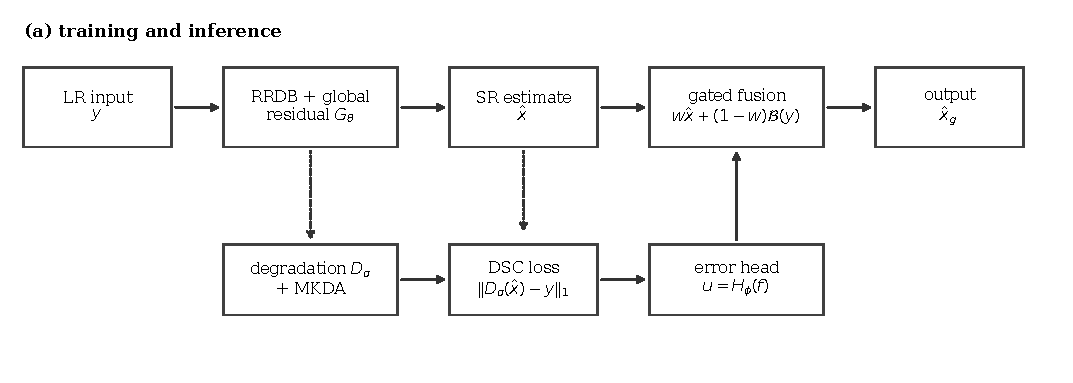
\includegraphics[width=0.92\textwidth]{fig_method.pdf}
\caption{Overview. The shared RRDB generator is trained with one of four configurations (L1, L1+Perc, L1+MKDA, L1+MKDA+DSC). At inference we study a training-free shrinkage toward bicubic, and compare it with a learned error-prediction gate. COP, illustrated separately in Fig.~\ref{fig:cop}, creates a flat reference region for evaluation.}
\label{fig:method}
\end{figure*}

\subsection{RRDB Training Configurations}
\paragraph{Pixel loss} $\mathcal{L}_{1}=\|G_\theta(y)-x\|_1$ is the conservative baseline.

\paragraph{Perceptual loss} $\mathcal{L}=\mathcal{L}_1+\lambda_p\| \phi(G_\theta(y))-\phi(x)\|_1$, with $\phi$ the first twelve layers of AlexNet and $\lambda_p=0.02$. This is the sharpness-oriented comparison.

\paragraph{Blur augmentation (MKDA)} Each mini-batch samples $\sigma\sim\mathcal{U}\{0.5,0.8,1.1,1.4\}$ and applies \eqref{eq:degradation} on the fly. This exposes the model to a range of simulated blur levels.

\paragraph{Degradation self-consistency (DSC)} We re-degrade the prediction and require it to reproduce the input:
\begin{equation}
\mathcal{L}_{\mathrm{DSC}} = \left\| \downarrow_s\!\left(k_\sigma * G_\theta(y)\right) - y \right\|_1 ,
\label{eq:dsc}
\end{equation}
and optimise $\mathcal{L}_1+0.5\,\mathcal{L}_{\mathrm{DSC}}$. DSC penalises errors that remain visible after re-degradation. High-frequency differences suppressed by degradation can have little effect on this penalty.

\subsection{Training-Free Risk Control}
A constant shrinkage toward bicubic,
\begin{equation}
\hat{x}_\alpha = \alpha\,\hat{x} + (1-\alpha)\,\mathcal{B}(y),\qquad \alpha\in[0,1],
\label{eq:shrink}
\end{equation}
interpolates between the SR estimate ($\alpha=1$) and bicubic interpolation ($\alpha=0$). The completed test comparison uses $\alpha=0.9$, and the validation sweep evaluates multiple blend weights. We also train a post-hoc error head $H_\phi$ on the frozen generator, with target $t=e/(e+\tau)$, $e=|\hat{x}-x|$, $\tau=0.02$, and gate the output as
\begin{equation}
w=e^{-\beta u},\qquad \hat{x}_{\mathrm{g}}=w\,\hat{x}+(1-w)\,\mathcal{B}(y),
\label{eq:gate}
\end{equation}
where $u=H_\phi(f)\in[0,1]$. The sweep selects a gate setting on validation and compares active gating with uniform blends at nearby HE values.

\subsection{Counterfactual Occlusion Probe}
COP requires no model modification. For a test slice $x$, we select $K$ textured $48\times48$ patches that lie inside the brain and whose mean gradient magnitude is above the 60th percentile of candidate patches. Each patch $P$ is replaced by its mean intensity,
\begin{equation}
x^{\mathrm{occ}}(p) = \begin{cases}\mu_P, & p\in P,\\ x(p), & \text{otherwise},\end{cases}
\end{equation}
and $y^{\mathrm{occ}}$ is obtained with \eqref{eq:degradation}. The model reconstructs $\hat{x}^{\mathrm{occ}}=G_\theta(y^{\mathrm{occ}})$. Inside the inner $32\times32$ region $\Omega\subset P$ (which excludes the patch seam), we define
\begin{equation}
\mathrm{HE} = \frac{\mathbb{E}_{p\in\Omega}|\nabla \hat{x}^{\mathrm{occ}}(p)|}{\mathbb{E}_{p\in\Omega}|\nabla x(p)|},
\qquad
\mathrm{VR} = \frac{\mathrm{std}_{\Omega}(\hat{x}^{\mathrm{occ}})}{\mathrm{std}_{\Omega}(x)}.
\label{eq:cop}
\end{equation}
For a flat output, these ratios are near zero with numerical stabilisation. A value near one indicates texture magnitude comparable to the unedited reference. The ratios can exceed one. We also report the mean absolute error to the flat reference (MAE). The probe is complemented by standard fidelity metrics on unmodified slices; none of them localises fabrication, which is why COP is reported alongside them.

\subsection{Proposed Paired Detail Recovery Error}
\label{sec:paired-metric}
HE quantifies structure in a region that should be flat. To measure the response to the original detail at the same location, we reconstruct both $x$ and $x^{\mathrm{occ}}$ after degradation with the same operator and, when applicable, the same noise realisation. We keep the intensity normalisation fixed between branches. Define the reference and output changes as
\begin{equation}
\Delta x = x-x^{\mathrm{occ}},\qquad
\Delta\hat{x} = \hat{x}-\hat{x}^{\mathrm{occ}}.
\end{equation}
For a field $v$, write $\|v\|_{1,\Omega}=\sum_{p\in\Omega}|v(p)|$. We propose the paired detail recovery error
\begin{equation}
\mathrm{PDRE} =
\frac{\|\Delta\hat{x}-\Delta x\|_{1,\Omega}}
     {\|\Delta x\|_{1,\Omega}+\epsilon},
\label{eq:pdre}
\end{equation}
where $\epsilon=10^{-6}$ stabilises the denominator for references scaled to $[0,1]$. Patch selection uses the unedited reference and is fixed before evaluating the outputs.

A response equal to $\Delta x$ gives PDRE zero. If the reconstructions are identical in $\Omega$, the score approaches one for patches with appreciable reference contrast. If the model recovers a fraction $a$ of the reference change at the correct location, the score is approximately $|1-a|$. A displaced edge or a sign reversal incurs error even when the response has the correct total magnitude. Because a structure shared by the two outputs cancels in the difference, we report PDRE alongside HE and check fidelity directly on the unedited branch. The pair of metrics distinguishes a flat response with low HE from a reconstruction that preserves the removed detail while also keeping the flat region flat.

\subsection{Proposed Fine-Tuning on Paired Inputs}
\label{sec:pair-training}
We propose starting from the pixel-loss RRDB checkpoint and constructing an original and flattened pair on the fly from training crops. Let $\ell_{\mathrm{flat}}$ be the mean gradient magnitude of $\hat{x}^{\mathrm{occ}}$ on the inner region, with the gradient stencil contained in the flat patch. We use the objective
\begin{equation}
\mathcal{L}_{\mathrm{pair}} =
\mathcal{L}_{1} + \lambda_f\ell_{\mathrm{flat}}
+ \lambda_r\,\mathrm{PDRE},
\label{eq:pair-loss}
\end{equation}
where $\mathcal{L}_{1}$ is the mean absolute reconstruction error on the unedited crop and the weights are nonnegative. The flat-branch loss penalises texture where the reference has none. The response loss penalises weakening, moving, or reversing the removed detail in the output difference. The unedited reconstruction loss anchors intensities and constrains structure shared by both outputs. The training scheme uses the same generator for both branches and requires only the standard SR forward pass at inference.

\section{Experiments}
\subsection{Data}
We use the public IXI T1w dataset \cite{ixi2007}, which contains 581 healthy adult volumes from three sites (Guys, HH, IOP). We randomly sample 72 subjects stratified by site. Each volume is brain-extracted with deepbet \cite{deepbet2024}, normalised with the 1st/99th percentile of brain voxels, and axially sliced. Slices with less than 10\% of the maximal brain area are discarded; the remaining slices are resampled to 1~mm isotropic and centre-padded to $256\times256$. The split is by subject: \numTrainSubjects{} training, \numValSubjects{} validation and \numTestSubjects{} test subjects (\numTrainSlices{}, \numValSlices{} and \numTestSlices{} slices), with no subject appearing in more than one split. The validation split is used for checkpoint selection and for comparing the blend controls.

\subsection{Training}
Models are trained for \numSteps{} iterations with Adam \cite{kingma2015adam} (learning rate $2\times10^{-4}$, cosine decay to $10^{-6}$, 200-step warm-up), batch size 8, and $192\times192$ HR patches ($48\times48$ LR). Augmentation consists of random crops, flips and $90^\circ$ rotations. Validation PSNR is computed every 500 iterations on 24 fixed validation slices, and the best checkpoint is kept. The four completed RRDB configurations use the same backbone and update budget. Training and evaluation run on a single Apple M3 Pro GPU (MPS) with PyTorch \numTorchVersion{}.

\subsection{Completed Comparisons}
\textbf{Bicubic} is the non-learned control. \textbf{RRDB} is the shared backbone with an $\ell_1$ loss. \textbf{RRDB+MKDA} adds multi-kernel augmentation. \textbf{RRDB+DSC+MKDA} adds both DSC and MKDA. \textbf{RRDB+Perc} adds the AlexNet perceptual loss. \textbf{RRDB+Shrink} applies \eqref{eq:shrink} to the pixel-loss model with the validation-selected $\alpha$. \textbf{RRDB+Gate} applies \eqref{eq:gate} to the frozen RRDB+DSC+MKDA model and is compared with a uniform blend of that same output on validation data.

\subsection{Metrics}
The completed experiments report PSNR, SSIM, mean LPIPS, HFEN (high-frequency error norm), and edge-SSIM for unedited references. COP reports HE, VR, and mean absolute error in flattened regions. We report LPIPS as an aggregate mean because the evaluation script stores this mean in each slice record. We interpret the archived slice and patch aggregates descriptively. The planned paired analysis uses subjects as the unit of comparison.

\subsection{Planned Evaluation}
\label{sec:planned}
\paragraph{Matched backbone comparison}
We will adapt HAT and MambaIRv2 to single-channel $\times4$ SR and compare them with RRDB and bicubic interpolation. We will keep the IXI subject split, pre-processing, LR inputs, training blur ($\sigma=0.8$), L1 loss, and validation checkpoint criterion common across the learned models. We will record model sizes, training budgets, and architecture-specific adjustments. Repeating the L1 versus L1-plus-perceptual-loss comparison within MambaIRv2 can test whether the effect observed in RRDB recurs in a second architecture.

\paragraph{Metric checks and independent fidelity measurement}
We will share the patch list across all methods, including bicubic. To check that the metrics respond to the intended errors, we will test ideal outputs and controlled modifications of the references. Adding texture only on the flat branch must increase HE. Returning the same flat output for both inputs must give low HE but high PDRE on textured patches. Shifting the original detail while keeping the flat branch fixed must increase PDRE relative to the ideal pair. We will assess sensitivity to the artificial patch seam by repeating the evaluation with a tapered transition outside $\Omega$ while preserving the constant interior. We will stratify the pairs by $\|y-y^{\mathrm{occ}}\|_2$, using cutoffs set on validation data, to distinguish interventions with weak LR evidence from those with a stronger measurable change.

On unedited slices, we will also measure local gradient error at a separately selected set of regions excluded from the paired evaluation. This check uses the gradient magnitudes and directions at corresponding positions:
\begin{equation}
 E_{\nabla} =
 \frac{\sum_{p\in\Omega}\lVert\nabla\hat{x}(p)-\nabla x(p)\rVert_2}
      {\sum_{p\in\Omega}\lVert\nabla x(p)\rVert_2+\epsilon},
 \label{eq:local-gradient}
\end{equation}
where $\epsilon>0$ stabilises the denominator. This check measures fidelity to anatomy in inputs where no region has been edited.

The training variants and the validation selection rule for suppression are specified in Section~\ref{sec:mitigation}.

\paragraph{Reporting}
We will plot HE against PDRE and report the unedited-region gradient error and slice-level fidelity separately. Each subject contributes its own mean across patches, and paired confidence intervals for method differences will be obtained by resampling subjects. Lower HE at comparable PDRE and without a material increase in unedited-region gradient error would support improved suppression at that operating point.

\section{Completed RRDB Results}

\subsection{Fidelity}
Table~\ref{tab:main} reports the in-distribution results at $\sigma=0.8$. Bicubic reaches \PSNRbic{}~dB. The pixel-loss RRDB improves PSNR to \PSNRrrdb{}~dB and LPIPS from \LPIPSbic{} to \LPIPSrrdb{}. MKDA and DSC+MKDA yield slightly lower PSNR than RRDB and higher PSNR than bicubic under the reference blur. The perceptual model attains the best LPIPS (\LPIPSperc{}) at a PSNR of \PSNRperc{}~dB. PSNR varies relatively little across the learned configurations, motivating separate examination of COP scores.

\begin{table*}[!t]
\centering
\caption{In-distribution results ($\times4$, $\sigma=0.8$). Mean over \numTestSlices{} test slices from \numTestSubjects{} held-out subjects. Arrows indicate the preferred direction.}
\label{tab:main}
\begin{tabular}{lccccc}
\toprule
Method & PSNR$\uparrow$ & SSIM$\uparrow$ & LPIPS$\downarrow$ & HFEN$\downarrow$ & Edge-SSIM$\uparrow$ \\
\midrule
Bicubic        & \PSNRbic{} & \SSIMbic{} & \LPIPSbic{} & \HFENbic{} & \EDGEbic{} \\
RRDB           & \PSNRrrdb{} & \SSIMrrdb{} & \LPIPSrrdb{} & \HFENrrdb{} & \EDGErrdb{} \\
RRDB+MKDA      & \PSNRrrdbmkda{} & \SSIMrrdbmkda{} & \LPIPSrrdbmkda{} & \HFENrrdbmkda{} & \EDGErrdbmkda{} \\
RRDB+DSC+MKDA  & \PSNRtrust{} & \SSIMtrust{} & \LPIPStrust{} & \HFENtrust{} & \EDGEtrust{} \\
RRDB+Perc      & \PSNRperc{} & \SSIMperc{} & \LPIPSperc{} & \HFENperc{} & \EDGEperc{} \\
RRDB+Shrink    & \PSNRshr{} & \SSIMshr{} & \LPIPSshr{} & \HFENshr{} & \EDGEshr{} \\
\bottomrule
\end{tabular}
\end{table*}

\subsection{Spurious Texture}
Table~\ref{tab:cop} and Fig.~\ref{fig:pareto} summarize the COP results. The archived bicubic control has COP energy \HEbic{} on 158 patches. The learned configurations use a common set of \ArchivePatches{} patches, allowing paired comparisons among them. The pixel-loss RRDB has HE \HErrdb{}. The perceptual model reaches \HEperc{}, a \HEpercPct{}\% increase relative to RRDB, alongside improved mean LPIPS. MKDA also increases HE (\HErrdbmkda{}), and adding DSC to MKDA raises it further (\HEtrust{}).

Uniform blending at $\alpha=0.9$ lowers HE to \HEshr{} (\HEshrinkPct{}\% below RRDB) with a global PSNR decrease of \PSNRshrink{}~dB. The corresponding change in local fidelity remains to be measured with \eqref{eq:pdre} and \eqref{eq:local-gradient}.

\begin{table}[!t]
\centering
\caption{COP and PSNR at additional test degradations. Lower HE and VR indicate less texture on flattened patches. Archived bicubic results use a separate patch set and a larger slice set in the additional degradation columns.}
\label{tab:cop}
\setlength{\tabcolsep}{2.8pt}
\begin{tabular}{lcccc}
\toprule
Method & HE$\downarrow$ & VR$\downarrow$ & PSNR$_{\text{blur1.4}}$ & PSNR$_{\text{bicubic}}$ \\
\midrule
Bicubic       & \HEbic{} & \VRbic{} & \OODblurBic{} & \OODbicBic{} \\
RRDB          & \HErrdb{} & \VRrrdb{} & \OODblurRrdb{} & \OODbicRrdb{} \\
RRDB+MKDA     & \HErrdbmkda{} & \VRrrdbmkda{} & \OODblurRrdbmkda{} & \OODbicRrdbmkda{} \\
RRDB+DSC+MKDA & \HEtrust{} & \VRtrust{} & \OODblurTrust{} & \OODbicTrust{} \\
RRDB+Perc     & \HEperc{} & \VRperc{} & \OODblurPerc{} & \OODbicPerc{} \\
RRDB+Shrink   & \HEshr{} & \VRshr{} & \OODblurShr{} & \OODbicShr{} \\
\bottomrule
\end{tabular}
\end{table}

\begin{figure}[!t]
\centering
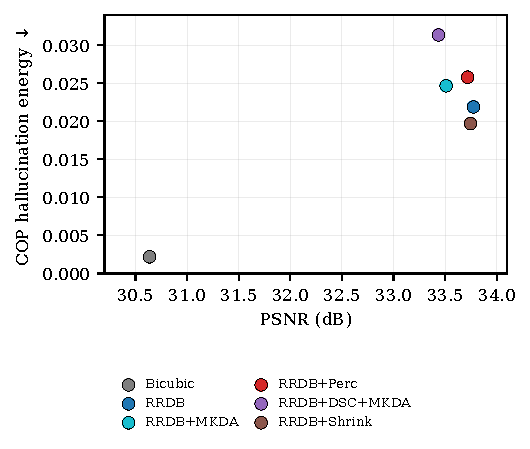
\includegraphics[width=\linewidth]{fig_pareto.pdf}
\caption{Test-set global PSNR and COP energy for the completed comparisons. Each point represents a model or output blend. The bicubic COP value uses a separate set of patches.}
\label{fig:pareto}
\end{figure}

\subsection{Subject-Balanced Reanalysis of Archived HE}
\label{sec:archive}
The archived means pool probe regions and therefore give more weight to subjects with more selected patches. We reanalysed the per-patch records by joining methods on subject, source slice, and patch coordinates. RRDB, Perc, MKDA, DSC+MKDA, and Shrink share \ArchivePatches{} probe regions from \ArchiveSubjects{} test subjects, with \ArchiveMinPatches{} to \ArchiveMaxPatches{} regions per subject (median \ArchiveMedianPatches{}). For each contrast we first computed the mean patch-level HE difference within each subject and then averaged over subjects. We resampled the \ArchiveSubjects{} subject-level differences with replacement \ArchiveBootstrapDraws{} times (seed \ArchiveBootstrapSeed{}) and report the central percentile interval. These intervals describe variation across test subjects for the archived checkpoints. They do not capture training-seed variability. Bicubic is excluded because its archived patch identifiers differ.

\begin{table}[!t]
\centering
\caption{Completed subject-balanced reanalysis. HE differences and descriptive 95\% bootstrap intervals are in thousandths. The last column counts subjects with a higher mean HE for the first method.}
\label{tab:subject-he}
\setlength{\tabcolsep}{3pt}
\begin{tabular}{@{}lrrc@{}}
\toprule
Comparison & $\Delta$HE & 95\% interval & Higher \\
\midrule
\ArchiveComparisonRows
\bottomrule
\end{tabular}
\end{table}

The direction of each contrast is unchanged by balancing subjects, and all \ArchiveSubjects{} subject means move in the same direction within each contrast (Table~\ref{tab:subject-he}). The largest increment relative to fixed-blur L1 is for DSC+MKDA. The most direct contrast for adding DSC is against MKDA, where the mean increment is $\ArchiveDSCIncrement{}\times10^{-3}$. The uniform blend of the L1 output lowers HE by $\ArchiveShrinkDecrease{}\times10^{-3}$. The reanalysis narrows an interpretation of the archived aggregate: the observed pattern is shared across the sampled subjects under these trained configurations. It still cannot show whether detail on the unedited branch was recovered or lost.

\subsection{Performance Across Simulated Degradations}
At $\sigma=1.4$, MKDA gains \OODgain{}~dB over the RRDB trained with fixed blur, and DSC+MKDA gains \OODgainTrust{}~dB. This blur was included in the MKDA training range. The comparison measures tolerance to stronger blur relative to the fixed-blur baseline. Table~\ref{tab:cop} and Fig.~\ref{fig:ood} also report results for alternative downsampling and noise conditions.

\begin{figure}[!t]
\centering
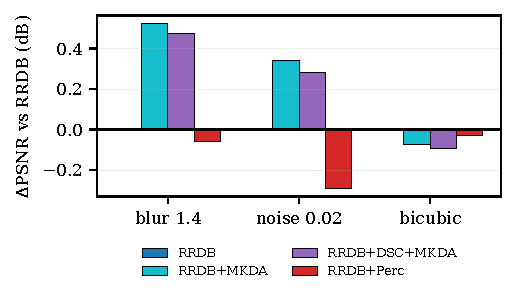
\includegraphics[width=\linewidth]{fig_ood.pdf}
\caption{PSNR under additional test degradations. The fixed-blur training uses $\sigma=0.8$. MKDA includes $\sigma=1.4$.}
\label{fig:ood}
\end{figure}

\subsection{Gate Versus Uniform Shrinkage}
In the validation sweep, the gate at $\beta=1$ has HE \HEgateOne{} and PSNR \PSNRgateOne{}~dB. The closest uniform blend on the sampled grid has HE \HEuniformOne{} and PSNR \PSNRuniformOne{}~dB. The settings are approximately matched on HE. The comparison gives the aggregate fidelity of these validation operating points.

\begin{table}[!t]
\centering
\caption{Validation comparison of the learned gate and a constant shrinkage at nearby COP scores.}
\label{tab:gate}
\begin{tabular}{lccc}
\toprule
Control & HE$\downarrow$ & PSNR & SSIM \\
\midrule
Gate $\beta=1$      & \HEgateOne{} & \PSNRgateOne{} & \SSIMgateOne{} \\
Shrinkage (nearest HE) & \HEuniformOne{} & \PSNRuniformOne{} & \SSIMuniformOne{} \\
\bottomrule
\end{tabular}
\end{table}

\subsection{Qualitative Results and Failure Cases}
Fig.~\ref{fig:qual} shows representative reconstructions and errors relative to the reference. Fig.~\ref{fig:cop} shows that the flattened regions remain nearly flat at display scale, with residual gradients captured by HE. Fig.~\ref{fig:failure} shows examples of residual error near small structures after blending under the standard simulated degradation.

\begin{figure*}[!t]
\centering
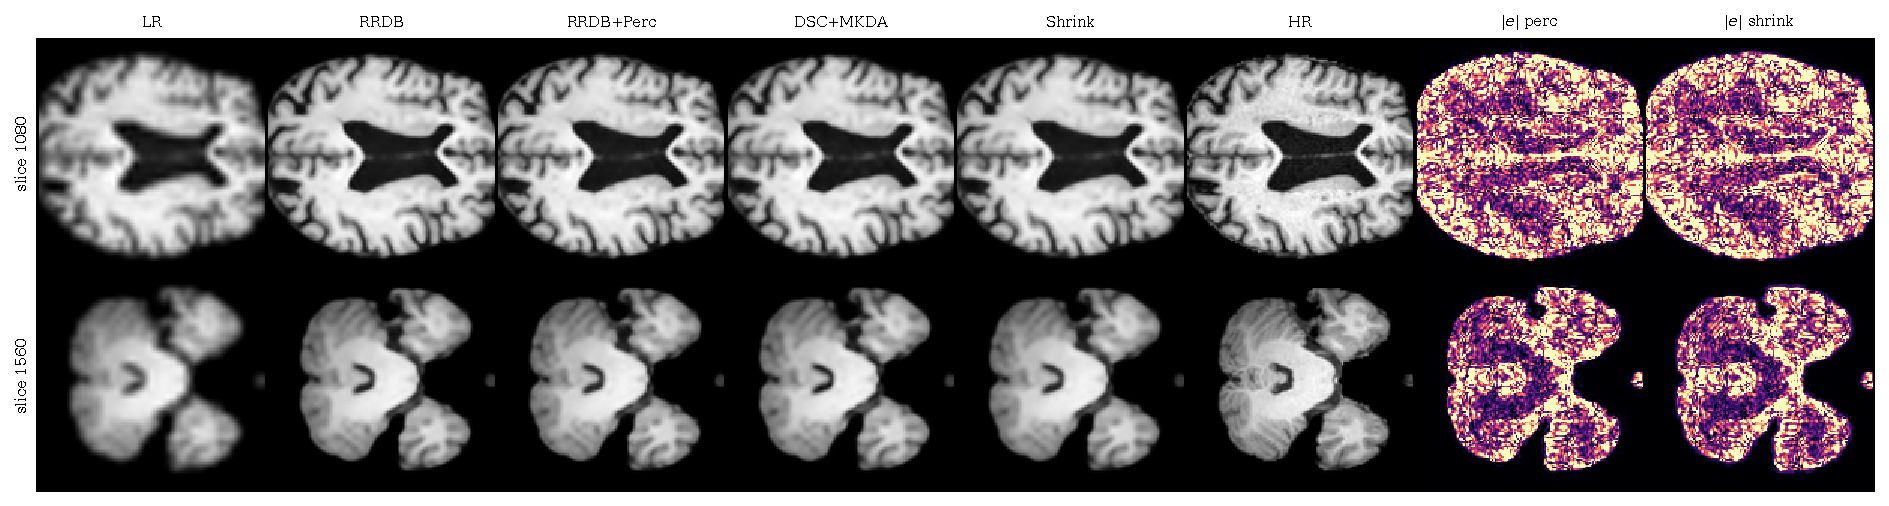
\includegraphics[width=\textwidth]{fig_qual.pdf}
\caption{Qualitative comparison ($\times4$). From left to right, bicubic-upsampled input, RRDB, RRDB+Perc, DSC+MKDA, uniform blend, HR reference, and absolute errors for Perc and the uniform blend.}
\label{fig:qual}
\end{figure*}

\begin{figure*}[!t]
\centering
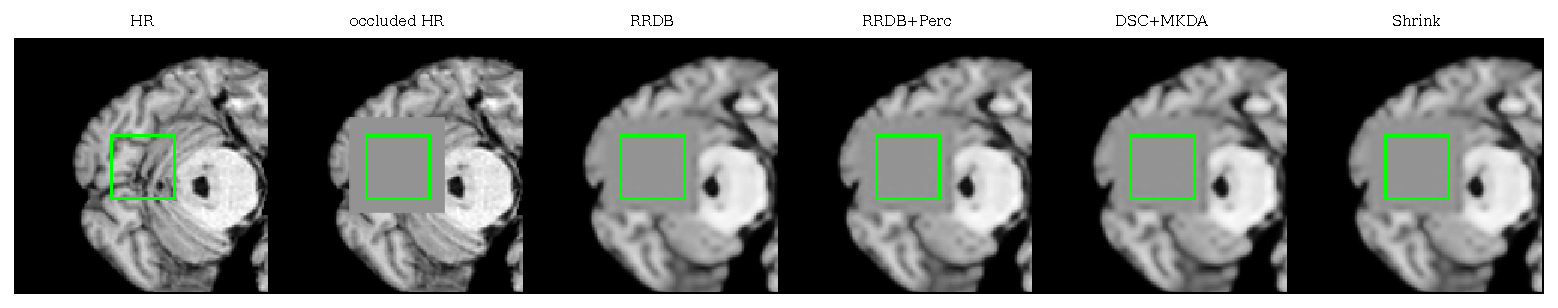
\includegraphics[width=\textwidth]{fig_cop.pdf}
\caption{Counterfactual occlusion probe. A textured patch is replaced by its local mean, degraded, and reconstructed; the inner region is outlined. All models leave the patch nearly flat, but the residual gradient energy differs, and that difference is what HE quantifies.}
\label{fig:cop}
\end{figure*}

\begin{figure}[!t]
\centering
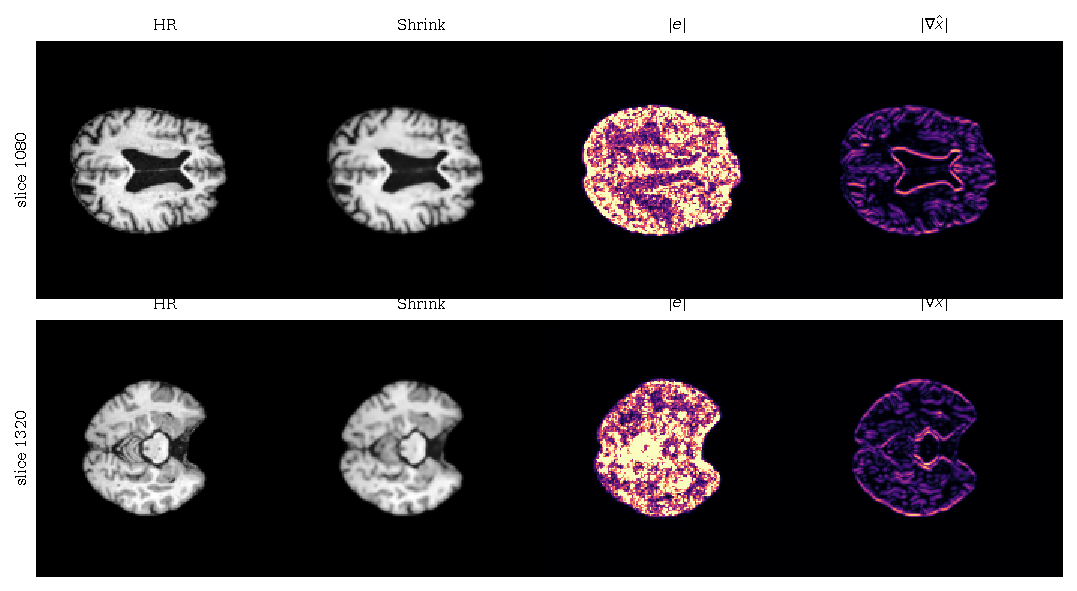
\includegraphics[width=\linewidth]{fig_failure.pdf}
\caption{Selected low-PSNR examples after blending, with the HR reference, absolute error, and output gradient.}
\label{fig:failure}
\end{figure}

\section{Ablation of the Evaluation Standard}
\label{sec:metric-ablations}
\subsection{What Each Score Can Identify}
Write $e_o=\hat{x}-x$ and $e_f=\hat{x}^{\mathrm{occ}}-x^{\mathrm{occ}}$ for the errors of the original and flat branches. Then $\Delta\hat{x}-\Delta x=e_o-e_f$. PDRE measures the difference of the errors, which is the part attributable to the change between the two inputs under this intervention. If the model adds the same error to both outputs, the difference vanishes. HE can expose a textured error shared by both branches because that error is still present on the flat output. A constant offset shared by both branches is invisible to both measures. We therefore retain flat-reference mean absolute error (flat MAE) and an original-reference intensity check as auxiliary measures.

We compare PDRE with two simplified response scores. The first drops the reference normalization and reports $\|\Delta\hat{x}-\Delta x\|_{1,\Omega}/|\Omega|$, the mean absolute response error. This preserves spatial alignment but puts more weight on high-contrast regions when errors are proportional to the reference detail. The second keeps normalization and drops pixelwise correspondence:
\begin{equation}
 E_{\mathrm{amp}} =
 \frac{\big|\,\|\Delta\hat{x}\|_{1,\Omega}-\|\Delta x\|_{1,\Omega}\,\big|}
      {\|\Delta x\|_{1,\Omega}+\epsilon}.
\label{eq:amplitude}
\end{equation}
It tests agreement of total response magnitude. The reverse triangle inequality gives $E_{\mathrm{amp}}\leq\mathrm{PDRE}$. When the two responses have the same magnitude but occupy different locations, the gap between these quantities can be large. We also compare with $E_\nabla$ on the original branch to check which failures a single-branch reference error detects.

\subsection{Completed Controlled Output Ablation}
We took \ControlRegions{} probe regions from the archived IXI slices (indices \ControlIndices{}) and substituted known outputs for the model predictions. The reference is the original crop paired with its archived flat version. The score region is the inner $32\times32$ square. The controls are an ideal pair, a completely erased response, half the original detail, a two-HR-pixel horizontal displacement, and reversal of the detail about the flat intensity with clipping to $[0,1]$. We also added a zero-mean cosine texture of amplitude 0.01 and period four HR pixels to the flat output alone or to both outputs. In the final control we subtracted 0.02 from both outputs. This test varies one error pattern at a time and uses no model training or inference. The scores describe the sensitivity of the evaluation, for the archived examples.

\begin{table*}[!t]
\centering
\caption{Completed metric ablation on controlled outputs made from \ControlRegions{} archived IXI reference regions. Mean scores over the regions. Response MAE and flat MAE are in thousandths of the normalized intensity. The small ideal HE is the numerical floor of the archived Sobel implementation.}
\label{tab:metric-controls}
\begin{tabular}{lrrrrrr}
\toprule
Controlled output pair & HE & PDRE & Amplitude error & Response MAE & Original gradient error & Flat MAE \\
\midrule
\ControlledAblationRows
\bottomrule
\end{tabular}
\end{table*}


\begin{figure*}[!t]
\centering
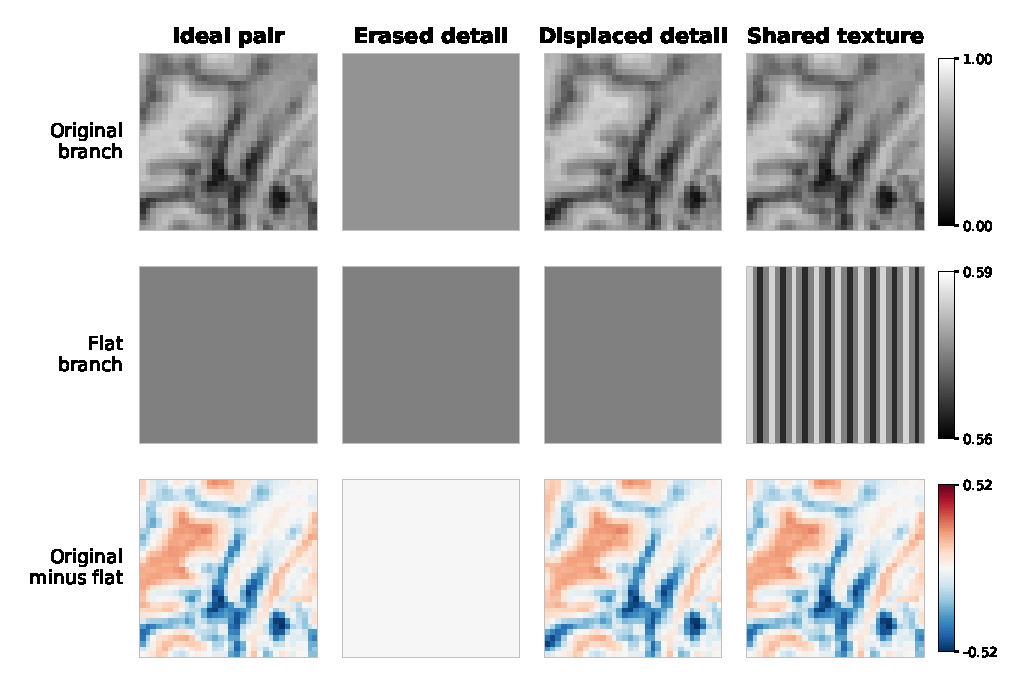
\includegraphics[width=0.95\textwidth]{fig_paired_controls.pdf}
\caption{Controlled outputs for one archived IXI probe region (slice index \ControlPreviewIndex{}). The top row shows the original branch and the middle row the flat branch. The middle row uses a narrow intensity window centred on the reference flat value to show the added texture. The bottom row shows the signed output difference with one scale across all columns. A two-pixel displacement moves the detail in the response. Texture added identically to both branches disappears in the difference but is visible in the flat output. These panels are controlled edits of the references.}
\label{fig:paired-controls}
\end{figure*}

Table~\ref{tab:metric-controls} shows where a reduced standard would give an incomplete account. With HE alone, an erased response and the ideal pair score the same. Replacing PDRE with the magnitude-only score makes a two-pixel displacement look close to ideal (\ControlShiftAmplitude{}), even though the pixelwise response error is \ControlShiftPDRE{}. The contrast-reversal example exhibits the same failure. With PDRE alone, adding the same texture to both outputs appears ideal, while HE increases from \ControlIdealHE{} to \ControlSharedHE{}. The corresponding output and difference images are shown in Fig.~\ref{fig:paired-controls}. In the offset control, the two primary scores stay at their ideal levels and flat MAE records the bias. These cases motivate reporting the two axes and the accompanying fidelity checks separately.

To isolate the normalization, we also repeated the half-amplitude error with the reference detail scaled by $1$ and $0.5$. Response MAE changed from \ControlContrastFullMAE{} to \ControlContrastHalfMAE{}, while PDRE remained \ControlContrastPDRE{} after rounding. Normalization therefore makes equal fractional attenuation comparable in this controlled case. On real data it can amplify errors for nearly flat reference changes. The reference-based eligibility criterion, the distribution of denominators, and a low-contrast sensitivity analysis are part of the planned evaluation.

\subsection{Planned Ablations on Model Outputs}
\label{sec:planned-metric}
The controlled test establishes which errors the formulas can detect by construction. The full ablation will use a fixed set of learned and bicubic outputs, which allows alternative scores to be recomputed without retraining. The question is whether each component changes the interpretation of a real comparison. For example, if the model ranking based on HE changes once detail recovery is considered, the relevant evidence is the model-by-model pair of differences on the same subjects. A score correlation alone cannot establish whether either score can distinguish a particular failure.

\begin{table*}[!t]
\centering
\caption{Planned metric ablation. Change one component at a time and reuse the same subject split, model outputs, and patch identifiers wherever the intervention permits.}
\label{tab:metric-ablation}
\small
\begin{tabular}{@{}>{\raggedright\arraybackslash}p{.17\textwidth}>{\raggedright\arraybackslash}p{.32\textwidth}>{\raggedright\arraybackslash}p{.45\textwidth}@{}}
\toprule
Component & Comparison & Evidence to examine \\
\midrule
Two-axis reporting & HE alone, PDRE alone, and HE with PDRE & Frequency of low-HE but poor-recovery cases and low-PDRE cases with texture on the flat branch \\
Spatial correspondence & Pixel-aligned PDRE versus amplitude error & Underestimation of displaced or reversed detail by the magnitude-only score \\
Reference normalization & PDRE versus unnormalized response MAE & Whether weak- and strong-contrast patches tell a consistent story about relative detail loss \\
Original-branch reference & PDRE versus gradient error and local MAE on unedited inputs & Disagreements that reveal common-mode errors or low-frequency intensity bias \\
Flattening boundary & Hard seam versus cosine taper outside the flat interior & Whether model differences survive removal of the sharp artificial seam \\
Spatial support & Inner squares of 24, 32, and 40 HR pixels for a fixed hard $48$-pixel patch & Whether extending the evaluation toward the seam changes the measured effect \\
Reference selection & Standard texture criterion versus lower and higher gradient strata & Stability across contrast and spatial scale, with the low-signal stratum reported separately \\
Noise pairing & Same noise in both branches versus independent noise as a stress test & Sensitivity of the response to a change in the noise realization, using repeated draws \\
\bottomrule
\end{tabular}
\end{table*}

For the taper variant, we will retain the same flat value through the inner 32 pixels and transition to the unedited reference across the eight-pixel border of the $48\times48$ patch. Scores for the two seam conditions will be compared on the same inner support. The size sweep will separately vary the scored support inside the hard patch. In the contrast analysis, patch strata will be defined using the unedited references and fixed before looking at model scores. We will also report LR change strength within each stratum. A low-contrast HR detail may be retained in LR, and a high-contrast fine pattern may be substantially removed, so the two stratifications address different sources of uncertainty.

All variants will be assessed by within-subject differences and the fraction of subjects for which the direction of each comparison agrees with the primary setting. If a claimed improvement reverses when a taper or smaller core is used, we will report that it depends on the probe geometry. PDRE on shared-noise pairs is the primary noisy evaluation. The independent-noise variant deliberately measures the additional variability induced by changing both the detail and the noise. Direct unedited-region fidelity remains an independent check because the proposed training uses a form of PDRE as a loss.

\section{Mechanistic Interpretation}
\label{sec:mechanisms}
We distinguish the mechanism of a method from the explanation of its observed score. A reconstruction loss determines which errors are directly penalised. Its effect after training also depends on the distribution of LR inputs, the optimisation trajectory, and model capacity. The comparisons below identify what can be inferred from the archive and specify interventions that could test each proposed explanation.

\subsection{Bicubic Interpolation and Pixel-Loss RRDB}
Bicubic interpolation combines a local neighbourhood of LR samples without a learned prior. It transfers edges that are still visible in LR, but it has little basis for estimating structure removed by blur and pooling. Interpolation can also spread an intensity change across the flat-patch boundary or create overshoot near a sharp edge. These two effects predict low interior HE under favourable conditions and relatively high detail loss for fine structures. The archived control reaches \PSNRbic{}~dB on the reference degradation. Its HE is small on the archived bicubic patches, but the sample mismatch limits direct interpretation. The matched rerun should separate interpolated texture from learned texture by comparing the interpolation, the complete RRDB output, and the RRDB residual $r=\hat{x}-\mathcal{B}(y)$ on both branches. We will stratify by LR visibility and distance to the probe seam. This reveals whether a low HE arises from an intrinsically flat input interior or from limited ability to respond to surviving structure.

The fixed-blur RRDB increases PSNR by 3.13~dB over bicubic and improves the slice-level fidelity metrics at $\sigma=0.8$. The residual architecture begins at the interpolation solution and learns a correction conditional on the LR context. With unlimited capacity, minimising expected pixel-wise L1 yields a conditional median at each pixel. When the LR data are compatible with several locations of a thin boundary, many pixels in that boundary need not be present in the median prediction. This explains how a model can improve average fidelity while attenuating a particular fine edge. A learned prior can also produce a small residual on the flat branch when surrounding structures resemble patterns seen in the training data. High HE on that branch and weak PDRE on the original detail are therefore both possible with L1 training. Comparing the residual on the flat branch against the output difference on the paired branch directly tests whether the learned correction increases genuine detail, spurious texture, or both.

\subsection{Perceptual Loss}
The perceptual branch compares AlexNet activations between the prediction and the reference. The activations depend on local neighbourhoods and need not respond equally to a feature's presence, amplitude, and exact placement. A nearby or stronger edge can improve feature agreement without restoring the edge at the reference position. The archived Perc model reduces LPIPS from \LPIPSrrdb{} to \LPIPSperc{} and raises HE by \HEpercPct{}\%. The subject-balanced comparison in Table~\ref{tab:subject-he} shows that this direction is shared across the sampled subjects. LPIPS also uses AlexNet features, although it uses its own scaling and learned weights. Agreement between the training feature loss and a feature-based test metric therefore provides limited evidence about independent anatomical fidelity.

A test of the feature-prior explanation will vary $\lambda_p\in\{0,0.01,0.02,0.04\}$ with the architecture, training degradations, initialisation seeds, and update budget held common. Evaluation will compare HE, PDRE, and original-branch gradient error by reference contrast and by LR detail strength. An increase in HE accompanied by lower PDRE would support a trade-off in which the feature loss recovers some detail while also producing additional texture. Rising HE with stable or worse PDRE would favour the explanation that it increases apparent texture without recovering the removed detail. A complementary comparison will inspect positions where the output develops an edge on the flat branch and check whether a matching edge is actually present at the same position in the original reference. This prevents improved slice-level LPIPS from serving as the only evidence for the claimed benefit.

\subsection{Multi-Kernel Degradation Augmentation}
MKDA samples the blur level during training. Its improvement under $\sigma=1.4$ is consistent with exposure to that blur. At the reference blur of $0.8$, the same model gives lower PSNR and higher HE than fixed-blur L1. A shared model without an explicit kernel input must learn a mapping across all blur levels. Similar LR observations can arise from weak HR edges under mild blur or strong HR edges under heavier blur. The pooled training distribution can therefore increase ambiguity about the necessary correction. Another possible factor is allocation of the fixed update budget across four blur values. The current results do not separate ambiguity from allocation.

A diagnostic comparison will train fixed-blur controls at $0.8$ and $1.4$, with the same total updates, and test both controls and the mixed model at both blur values. A second mixed model supplied with the blur level as an input would test whether explicit conditioning removes part of the HE increase. Its parameter count, preprocessing, and training budget will be documented. If explicit conditioning narrows the gap at the reference blur while retaining stronger-blur fidelity, the unknown-kernel explanation becomes more plausible. If a longer mixed training run narrows the gap while conditioning has little effect, optimisation or sample allocation becomes a more plausible contributor. Reporting both HE and PDRE at each blur separates adaptation to the degradation from improved recovery of actual detail.

\subsection{Degradation Self-Consistency}
For the noise-free linear blur-and-pool operator $D_\sigma$, replacing $\hat{x}$ with $\hat{x}+h$ changes the consistency residual by $D_\sigma h$. The reverse triangle inequality gives
\begin{equation}
\begin{split}
&\big|\|D_\sigma(\hat{x}+h)-y\|_1
           -\|D_\sigma\hat{x}-y\|_1\big|\\
&\hspace{3em}\leq \|D_\sigma h\|_1.
\end{split}
\label{eq:dsc-bound}
\end{equation}
For an alternating high-frequency pattern, positive and negative contributions can cancel under averaging. In such a case the HR perturbation can be large while the LR change is small. Thus an image can satisfy the LR constraint and still contain texture errors \cite{bhadra2021hallucinations}. This argument explains why the constraint has limited leverage on certain errors. Explaining the observed HE increase over MKDA requires evidence about the trained solution, including whether DSC actually reduced the LR residual.

A factorial comparison will cross fixed and mixed blur with DSC off and on. This adds the missing fixed-blur L1+DSC cell and allows the effect of adding DSC to be compared at both training regimes. An initial sweep within the mixed regime will test weights $0$, $0.25$, and $0.5$. We will measure the re-degradation error of the unedited and flattened outputs separately, along with HE and PDRE. On the flat branch, we will also apply $D_\sigma$ to a smoothly windowed version of the local error and measure the amount that survives. A small LR residual with high HE and weak survival of that error would support the proposed explanation. A larger LR residual with high HE would instead point toward optimisation or model mismatch. The same evaluation with several seeds can show whether the archived increase is reproducible.

\subsection{Uniform Blending}
For fixed $\alpha$, the blend changes the paired response as
\begin{equation}
\Delta\hat{x}_\alpha =
\alpha\Delta\hat{x}+(1-\alpha)\Delta\mathcal{B},
\end{equation}
where $\Delta\mathcal{B}=\mathcal{B}(y)-\mathcal{B}(y^{\mathrm{occ}})$. Since the interpolation and learned output are clipped before blending, a convex combination stays within the same range. On the flat branch this operation scales the learned residual toward zero. It can reduce HE when that residual contributes spurious edges. It can also weaken true edges on the original branch if the residual is what restores them. If the learned residual itself displaces a boundary, reducing it could instead improve local fidelity. Thus the direction of PDRE under blending depends on the two response errors and can differ across patches.

At $\alpha=0.9$, the archived uniform blend lowers HE on all \ArchiveSubjects{} subjects relative to the same L1 generator. The global PSNR drop of \PSNRshrink{}~dB describes the slice average and gives limited information about edge preservation. The proposed diagnostic will evaluate the entire grid of blend weights on the same pairs, including $\alpha=0$ and $1$. We will examine the curve by LR visibility stratum and trace representative patches along it. In particular, a curve that reaches low HE only with high PDRE would show that global shrinkage suppresses both types of detail for that subset.

\subsection{Learned Error Gate}
The gate is trained to predict absolute reconstruction error. A slightly shifted, genuine edge can have high absolute error around the shift, so the target can also attenuate useful but imperfectly placed residuals. In a continuous approximation to the output $\mathcal{B}+wr$, the gradient includes $w\nabla r+r\nabla w$. A rapidly varying gate can therefore introduce a spatial gradient even where the residual itself is slowly varying. In paired evaluation, the original and flattened input can receive different gates, so the fixed-weight response identity no longer applies.

In the archived validation sweep, $\beta=1$ reduces HE from 0.03118 to 0.02116 but reduces PSNR by 0.603~dB from the ungated setting. The nearest sampled uniform blend ($\alpha=0.7$) has PSNR 0.336~dB higher at slightly higher HE. Under the archive's prespecified 0.05~dB validation allowance, the selected gate setting was $\beta=0$. These values characterise this generator and gate target. To check what the spatial weighting contributes, we will compare the learned map against a constant gate, a spatially shuffled map with the same values, and a smoothed map. The constant and smoothed controls will also be compared at similar validation HE. If shuffling has little effect, the gate's distribution of weights may explain more than their spatial placement. If smoothing decreases HE without increasing PDRE, gate transitions may contribute to the error. The independent unedited-region check will measure whether genuine boundaries receive unusually strong attenuation.

\subsection{Cross-Architecture Hypotheses}
HAT and MambaIRv2 are planned comparisons, with no archived MRI result. HAT uses attention to combine spatial context, and MambaIRv2 mixes information through an attentive state-space design. Access to context can help recover a weak but supported boundary. It can also reproduce a typical surrounding pattern inside a region where that pattern was removed. We will use the same low-resolution inputs and paired metrics to distinguish these behaviours. A small optional context test will alter a surrounding annulus while fixing the central LR crop, with tapering applied outside the scored region. This tests how much the central output changes when the external context changes. A larger change would establish sensitivity to the intervention, with HE and PDRE showing whether that sensitivity is beneficial in the primary task. Architecture comparisons will be interpreted with parameter count, optimisation budget, and training-seed variation reported alongside the results.

\section{Testing the Proposed Mitigation}
\label{sec:mitigation}
\subsection{Constructing Training Pairs}
The proposed fine-tuning uses the training subjects and a pretrained L1 checkpoint. Candidate regions will be drawn from augmented training crops after flips and rotations so that both branches share the same coordinates. We will select at most one region per training crop for the primary experiment. Its outer support must lie inside the brain mask and leave room for the degradation kernel. The same intensity scale, degradation settings, crop boundary, and noise draw will be used in the two branches. Crops with no eligible probe will still contribute their unedited reconstruction loss. A sample from one subject will never be paired with a sample from another subject.

The flat term averages the magnitudes of the horizontal and vertical Sobel response over the core. For training, subtracting the constant numerical floor of the stabilised magnitude leaves the optimisation unchanged. The response term uses the PDRE definition in \eqref{eq:pdre}. We will average each auxiliary term over eligible regions in the minibatch before multiplying by its weight. The patch selection threshold, retained fraction of eligible regions, and median reference-change norm will be recorded. If few low-contrast details are eligible, those data will be analysed as a separate test stratum rather than interpreted as evidence of training coverage.

Because $\Delta\hat{x}-\Delta x=e_o-e_f$, the response loss can be small when both branches make the same error. The original reconstruction term discourages that solution. Conversely, the flat term alone can favour an output that suppresses both useful and spurious gradients. Retaining the response term makes that strategy costly whenever the reference pair differs. These properties motivate the joint objective and explain why each component needs its own ablation.

\subsection{Loss Ablation and Matched Operating Points}
\begin{table}[!t]
\centering
\caption{Planned loss ablation from the same L1 checkpoint. Each fine-tuned variant includes the original-image L1 term.}
\label{tab:loss-ablation}
\setlength{\tabcolsep}{3pt}
\begin{tabular}{@{}lccc@{}}
\toprule
Variant & L1 & Flat term & Response term \\
\midrule
L1 continuation & Yes & Off & Off \\
Flat loss only & Yes & On & Off \\
Response loss only & Yes & Off & On \\
Full objective & Yes & On & On \\
\bottomrule
\end{tabular}
\end{table}

The four variants in Table~\ref{tab:loss-ablation} will share the original crops, update count, validation cadence, and fine-tuning seed. The same selected nonzero weights will be used in the full and single-term variants for the factorial comparison. We will first compare checkpoints after the same number of updates to measure the effect of the losses, then compare validation-selected operating points against frozen RRDB, uniform blending, and gating. This separates improvement due to additional optimisation from improvement due to paired supervision. Per-run wall time and the number of processed crops will be reported, since evaluating two branches adds work during training.

Let $P_0$ be the mean validation PDRE of frozen RRDB. For each mitigation, define eligible operating points by $\mathrm{PDRE}\leq P_0+\delta$, where $\delta$ is a tolerance fixed before testing. The primary comparison will use the setting with lowest validation HE among these points. If a method has no eligible setting, we will report that outcome and its curve. Each selected setting will then be evaluated on the same held-out pairs. Lower HE must be accompanied by a comparable PDRE and unchanged or improved fidelity on the independently selected unedited regions to support the intended conclusion. We will also report the outcome at zero allowance to show sensitivity to the choice of tolerance.

\subsection{Generalisation Beyond the Training Intervention}
The use of similar pairs at training and evaluation may favour a model that learns to recognise the synthetic edit. To investigate this, we will first train with hard mean replacement and evaluate the same checkpoints on tapered pairs. This isolates sensitivity to the seam. A second check will use the same locations in untouched images, with reference gradients and intensity errors computed directly. These results are the safeguards against declaring improvement based only on the same construction used in the loss. We will also inspect the original output, the flat output, and the signed response map in cases where PDRE and unedited fidelity disagree. A decline in HE that disappears under tapering or comes with worse unedited boundaries would limit the evidence for anatomical benefit.

\section{Limitations}
The completed experiments use two-dimensional T1-weighted slices from healthy adults and simulated in-plane degradation. HE measures residual gradients on the controlled flat region and can include ringing or other propagated errors. PDRE measures response to the specified intervention, including cases in which the LR difference is weak. Neither quantity establishes clinical lesion detection performance. The archived bicubic COP patch count differs from that of the learned configurations, so a matched rerun is required for direct comparison. The controlled output ablation covers \ControlRegions{} archived regions and establishes score behaviour for specified perturbations. Ranking trained methods by PDRE, measuring effects of paired fine-tuning, and establishing generalisation to other backbones require paired inference on the held-out subject set.


\subsection{From Probe Scores to Failure Cases}
To make the findings interpretable at the region level, we will show example pairs selected by prespecified score strata. For each backbone, the four strata will cross high or low HE with high or low PDRE. Cutoffs will be fixed from the L1 validation distribution and held common across methods. They provide a way to count cases and select representative examples, rather than clinical thresholds. We will report the number of test subjects with each pattern and show the corresponding reference difference, predicted difference, and unedited reconstruction. This analysis complements averages that may hide a subgroup whose detail is lost while the rest of the test set improves.

Disagreement between scores will guide the interpretation of mitigation. Low HE with high PDRE suggests that the model avoided adding texture in the flat region but failed to reproduce the removed detail. High HE with low PDRE can occur when the output responds correctly to the intervention while also placing a common false structure in both branches. High values on both axes can combine an inaccurate response with texture on the flat branch. A low-low case still warrants the independent intensity and gradient checks, especially if a bias or a shared structure is visible. These categories apply to the controlled intervention and cannot be assigned to an arbitrary scan without the paired reference.

\section{Conclusion}
In the completed RRDB experiments, a perceptual loss improved mean LPIPS while increasing texture in flattened COP regions. Blending with bicubic reduced COP energy with a small change in global PSNR. The subject-balanced archive reanalysis preserves the direction of these HE differences. Controlled ablations of the proposed PDRE and HE show how the two scores distinguish erased or displaced detail from spurious texture, while exposing errors that require an auxiliary fidelity check. We propose a paired fine-tuning objective to suppress spurious texture while retaining the response to genuine detail. Matched comparisons against blending and on unedited regions will determine whether the proposed objective preserves local anatomy at a comparable level of suppression.

\section*{Reproducibility}
Code, subject-level splits, and logs are available in the project repository. Running \texttt{python3 -m src.paired\_ablation} from the repository root reads the committed COP JSON and NPZ archives and regenerates the tables in Sections~\ref{sec:archive} and~\ref{sec:metric-ablations} and Fig.~\ref{fig:paired-controls}. This command requires NumPy and Matplotlib. The full MRI evaluation in Section~\ref{sec:planned} requires trained checkpoints and preprocessed slices.

\bibliographystyle{IEEEtran}
\IEEEtriggeratref{10}
\bibliography{refs}

\end{document}
